% Copyright \copyright\ 2010  Volodymyr Piven und Alexander Peltzer.
% Es wird die Erlaubnis gegeben, dieses Dokument unter den Bedingungen der von der Free
% Software Foundation veröffentlichen  GNU Free
% Documentation License (Version 1.2 oder neuer) zu kopieren, verteilen und/oder
% zu verändern. Eine Kopie dieser Lizenz ist unter
% http://www.gnu.org/copyleft/fdl.txt erhältlich.
%
% Copyright der Aktualisierung und Überarbeitung \copyright\ 2013  Simon Kalt, Jan-Peter Hohloch, Tobias Fabritz
% Es wird die Erlaubnis gegeben, dieses Dokument unter den Bedingungen der von der Free
% Software Foundation veröffentlichen  GNU Free
% Documentation License (Version 1.2 oder neuer) zu kopieren, verteilen und/oder
% zu verändern. Eine Kopie dieser Lizenz ist unter
% http://www.gnu.org/copyleft/fdl.txt erhältlich.
%
% Zusätzlich muss jede Kopie/Aktualisierung wieder über die Seite
% der Fachschaft Informatik der Uni Tübingen
% den Studenten zur Verfügung gestellt werden
% http://www.fsi.uni-tuebingen.de/

\chapter{Suchen in geordneten Mengen}
    Gegeben ist ein Universum $U$, mit linearer Ordnung $(U, <)$. Sei nun $S \subseteq U$ die Menge der zu verwaltenden Schlüssel. Wir betrachten nun verschiedene Algorithmen in $S$ ein Element zu suchen.
    \begin{enumerate}[1.] 
        \item \emph{lineare Suche:} $S$ liege als geordnetes Array vor. Nun sei next, das Element, das als nächstes betrachtet wird. \\
        Starte mit next $\leftarrow~0$\\
        Schleife: next $\leftarrow$ next $+~1$\\
        Abfrage: Ist $a~<~S\lbrack\text{next}\rbrack$?\\
        Laufzeit:\\
        best case: $\LO(1)$\\
        worst case: $\LO(n), n \text{ Iterat.}, |S| = n$\\
        average case: $\frac{n}{2}$ Iterat. $= \LO(n)$
        \item \emph{binäre Suche}: $S$ liege wieder als sortiertes Array vor. 2 Grenzen oben , unten als Indizes. Wir suchen wie in \autoref{alg:binarySearch} beschrieben.\\
            \begin{algorithm}
        		\caption{Binary Search}
        		\label{alg:binarySearch}
        		\begin{algorithmic}[1]
        			\Function{Suche}{$a,S$}
        			    \State $\text{unten} \gets 0$
        			    \State $\text{oben} \gets (n-1)$ \Comment{Array enthält $n$ Elemente}
        				\While{$\text{unten} < \text{oben}$}
        				    \State{$\text{next} \gets \lceil \frac{\text{oben} - \text{unten}}{2} \rceil + \text{unten}$}
                            \If{ $S[\text{next}] = a$ }
                                \State{\Return $\text{next}$}
                            \ElsIf{$S[\text{next}] < a$}
                                \State{$\text{unten} \gets \text{next}+1$}
                            \Else 
                                \State{$\text{oben} \gets \text{next}-1$}
                            \EndIf    
        				\EndWhile
        				\State \Return $-1$
        			\EndFunction
        		\end{algorithmic}
        	\end{algorithm}
        Laufzeit (best case): $T(n) = 1$ (zu suchendes Element genau in der Mitte)\\
        Laufzeit (worst case): 
        \begin{align*}
            T(n)~&=~1~+~T \left( \frac{n}{2} \right)\\
            &=~1~+~1~+~T \left( \frac{n}{4} \right)\\
            &=~1~+~1~+~1~+~T \left( \frac{n}{8} \right)\\
            &=~i~+~T \left( \frac{n}{2^{i}} \right)\tag{i-ter Schritt}\\
            &=~\log n~+~T(1)~=~O \left( \log n \right)
        \end{align*}
    \end{enumerate}

    \section{Interpolationssuche}

        next $\leftarrow~\left\lfloor \frac{a - S \lbrack \text{unten} \rbrack}{S \lbrack \text{oben} \rbrack - 
        S \lbrack \text{unten} \rbrack} \cdot \left( \text{oben} - \text{unten} \right)\right\rfloor + \text{unten}$\\
        \begin{tabbing}
            Laufzeit: \= worst case: $\LO(n)$\\
            \> average case: $\LO(\log \log n)$\\
        \end{tabbing}

        \begin{figure}
            \centering
            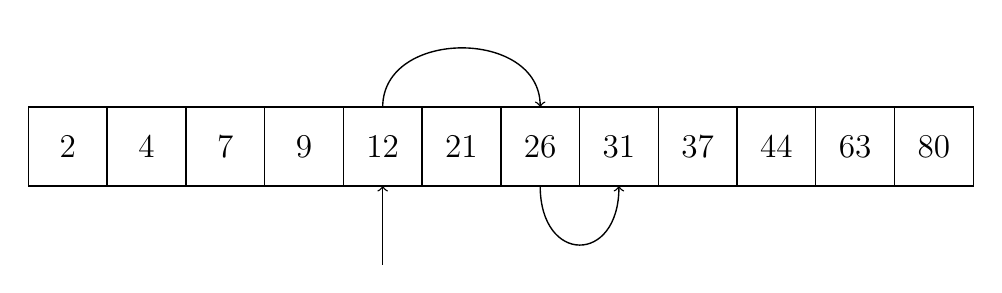
\begin{tikzpicture}[->,node distance=1cm, box/.style={draw,shape=rectangle,minimum size=1cm,font=\large},line width=0.5pt]
    \node[box] (1) at (0,0) {2};
    \node[box] (2) [right of=1] {4};
    \node[box] (3) [right of=2] {7};
    \node[box] (4) [right of=3] {9};
    \node[box] (5) [right of=4] {12};
    \node[box] (6) [right of=5] {21};
    \node[box] (7) [right of=6] {26};
    \node[box] (8) [right of=7] {31};
    \node[box] (9) [right of=8] {37};
    \node[box] (10) [right of=9] {44};
    \node[box] (11) [right of=10] {63};
    \node[box] (12) [right of=11] {80};

    \draw (4,-1.5) -- (4,-0.5);
    \draw (4,0.5) .. controls +(90:1) and +(90:1) .. (6,0.5);
    \draw (6,-0.5) .. controls +(-90:1) and +(-90:1) .. (7,-0.5);
\end{tikzpicture}

            \caption{Interpolationssuche}
            \label{diag2:interpolationsearch}
        \end{figure}
        
        Interpolieren und Springen sukzessive in Sprüngen der Länge $\sqrt{\text{oben} - \text{unten}}$, bis das richtige Suchintervall gefunden ist.
        Suchintervall hat Größe $\sqrt{\text{oben} - \text{unten}}$.

    
    \section{Erweiterung der Suche in geordneten Mengen}
        $\btl S \btr = n$ \\
        \begin{enumerate}[a.)]
            \item Lineare Suche $\LO(n)$ 
            \item Binäre Suche $\LO(\log n)$
            \item Interpolationssuche $\LO(\log \log n)$ im Mittel.
        \end{enumerate}
      
        \subsection{Variante von Reingold}
            $S$ als Array $S\lbrack 1 \rbrack, \ldots, S \lbrack
            n \rbrack$ füge künstliche Elemente ein $S \lbrack 0 \rbrack, \ldots S
            \lbrack n+1 \rbrack$ \\
            next $\leftarrow$ (unten -1) + $\lceil \frac{a-S(\text{unten}
            -1)}{S(\text{oben} +1) - S (\text{unten}-1)} \cdot (\text{oben - unten} + 1) \rceil$ \\
            Starte mit $n \leftarrow$ oben $-$ unten $+1$\\
            \begin{enumerate}[(1)]
                \item
                Interpoliere: $a : S[next]$ 
                \item 
                falls ``='' fertig \\
                falls $>$: lineare Suche in $S[next+\sqrt{n}], S[next+2 \cdot \sqrt{n}] \cdots \ \text{ bis } a < S[next+(i-1)\sqrt{n}]$ \\
                Es gilt : Nach $i$ Vergleichen gilt: $S[next+(i-2)\sqrt{n}) \leq a < S[next+(i-1)\sqrt{n}]$ \\
                falls $<$: analoges Vorgehen
                \item
                rekursiv im Suchintervall der Größe $\sqrt{n}$ weitersuchen. \\
            \end{enumerate}
        
        \subsection{Analyse}
            Sei $C$ die mittlere Anzahl von Vergleichen um auf Teilproblem der Größe $\sqrt{n}$ zu kommen, dann: \\
            \begin{align*}
                T(n) &\leq C + T(\sqrt{n}) \\
                T(1) &= 1 \\
				T(2) &= 1 \\
                T(n) &= \LO(\log \log n) \text{falls } C \text{ konstant.}
            \end{align*}
            Berechnung:
            \begin{align*}
                T(n) &= C + T(\sqrt{n})  \\
                &= C + C + T\left(n^{\frac{1}{4}}\right) \\
                &= ... = \\
                &= i \cdot C + T\left(n^{\frac{1}{2^i}}\right) \overset{!}{=} a \cdot C + T(2)
            \end{align*}
            Nun soll berechnet werden für welches $a$ gilt:
            \begin{align*}
                n^{\frac{1}{2^{a}}} &= 2 \\
                \log n^{\frac{1}{2^{a}}} &= log 2 \\
                \frac{1}{2^{a}}\cdot \log n &= 1 \\
                \log n &= 2^{a} \\
                \log{ \log n} &= a
            \end{align*}
        
            \subsubsection{Wahrscheinlichkeitsannahme}
                Elemente $a_1 \ldots a_n$ und auch $a$  sind zufällige Elemente aus ($a_0, a_{n+1}$) gezogen nach Gleichverteilung. \\
                Sei $p_i$ Wahrscheinlichkeit, dass $\geq i$ Vergleiche nötig sind. \\
                $\Ra C_i = \sum_i i \cdot  \underbrace{(p_i - p_{i+1})}_{\text{Prob(genau i Vergleiche.)}} 
                		=1(p_1 - p_2) + 2(p_2 - p_3) + 3(p_3-p_4) = \sum \limits_{i \geq 1} p_i$ \\
                \newline
                $p_1 = 1 = p_2$ \\
                Was ist jetzt $p_i$ ? \\
                Falls $i$ Vergleiche nötig sind, weicht der tatsächliche Rang von $a$ in der Folge $a_1 , \ldots, a_n$ um mindestens 
                		$(i-2) \cdot \sqrt{n}$ von next ab. \\
                (Rang von a: Anzahl von $a_i$ mit $a_i < a$) \\
                das heißt: $p_i \leq \text{ prob } ((Rang(a) - next) \geq (i-2) \sqrt{n})$ \\
                bedeutet $\text{ prob } ((y - \mu (y)) \geq (i-2) \cdot \sqrt{n})$ mit unten = 1, oben = n, next = $p \cdot n$ \\
                $p = \frac{a-S[unten -1 ]}{S[oben+1] - S[unten - 1 ]}$\\
                \newline
                next ist die erwartete Anzahl der Elemente $\leq a$ \\
                also der erwartete Rang von $a$. \\
                Sei $y$ Zufallsvariable, die Rang von $a$ in $a_1, \ldots, a_n$ angibt, sowie $\mu(y)$ Erwartungswert. \\\\
                \textit{Tschebyscheff'sche Ungleichung:}
                $$\text{ prob } ((y- \mu (y)) > t) \leq \frac{Var(y)}{t^2}$$
                $Var(x) = E((x-E(x))^{2})$ 
            

                \begin{tabbing}
                    Es gilt: \= Erwartungswert: $p \cdot n$\\
                    \> Varianz: $(1-p)\cdot p \cdot n$
                \end{tabbing}
                    Erwartungswert $\mu$\\
                prob( genau j Elemente < a) = $\begin{pmatrix}
                                n \\ j
                                           \end{pmatrix} p^{j} (1-p)^{n-j}$\\
                Deshalb: 
                \begin{align*}
                    \mu &= \sum \limits_{j=1}^{n} j \cdot \begin{pmatrix}
                    n \\ j
                    \end{pmatrix} p^{j} (1-p)^{n-j}\\
                    &= n \cdot p \cdot \sum \limits_{i=1}^{n} \begin{pmatrix}
                    n-1 \\ j-1
                    \end{pmatrix} p^{j-1} (1-p)^{n-j}\\
                    &= n \cdot p \cdot \sum \limits_{j=0}^{n-1} \begin{pmatrix}
                    n-1 \\ j
                    \end{pmatrix} p^{j} (1-p)^{n-(j+1)}\\
                    &= n \cdot p \cdot 1\\
                    &= n \cdot p
                \end{align*}
                $p_i \leq$ prob $\left( \underbrace{Rang}_{y}~-~\underbrace{next}_{\mu}~\geq~\underbrace{(i-2) \sqrt{n}}_{t} \right)$\\
                $\leq \frac{Var(y)}{t^2} = \frac{p(1-p)\cdot n}{(i-2)^{2} \cdot n} 
                	\overset{p\cdot(1-p)\leq \frac{1}{4}}{\underset{\text{da } 0\leq p\leq 1}{\leq}} \frac{1}{4(i-2)^{2}}$
            
                Es gilt
                $$
                    C \leq \sum_i p_{i} \leq 2 + \sum \limits_{i \geq 3} \frac{1}{4(i-2)^{2}} 
                    \leq 2+\frac{1}{4}\sum_{i\geq 1}{\left(\frac{1}{i}\right)^2}
                    \leq 2 + \frac{\pi^{2}}{24} \approx 2.4
                $$
                Im Mittel brauchen wir also $\LO(\log\log n)$ Versuche, da $T(n)=2.4 \log \log (n)$ \\
                \underline{worst case:} \\
                $T_{\text{worst}} (n) = T_{\text{worst}} (\sqrt{n}) + (\sqrt{n} +1) = 
                O\left(\sqrt{n}+ \sqrt{\sqrt{n}} + \sqrt{\sqrt{\sqrt{n}}}+\ldots \right) = \LO(\sqrt{n})$\\
                Es sind also $\sqrt{n}$ Sprünge nötig um Problem auf Größe $\sqrt{n}$ zu bringen.
                aber: Annahme der Gleichverteilung kritisch.
